\section{Results}

\begin{frame}{Scaling Law}
	\begin{figure}
		\centering
		% Pareto frontier — copied from yolo26-rfdetr-fml/figures/model-params-perf.tex
% Adapted for Beamer: bare tikzpicture (slide supplies figure env + caption + label).
\begin{tikzpicture}
\begin{axis}[
    width=0.92\linewidth,
    height=5.9cm,
    xlabel={Parameters (millions)},
    ylabel={$mAP_{50}$},
    xmode=log,
    xmin=1.5, xmax=150,
    ymin=0.74, ymax=0.86,
    xtick={2, 5, 10, 20, 40, 100, 150},
    log ticks with fixed point,
    ytick={0.74, 0.76, 0.78, 0.80, 0.82, 0.84, 0.86},
    ymajorgrids=true,
    grid style={dashed, gray!30},
    legend pos=south east,
    legend style={font=\footnotesize, cells={anchor=west}, draw=gray!30, rounded corners=1pt},
    tick label style={font=\footnotesize},
    label style={font=\small},
]
\addplot[
    color=softblue!80!black,
    mark=square*,
    mark options={fill=softblue, draw=softblue!80!black},
    thick,
]
coordinates {
    (4.1, 0.7659)
    (32.1, 0.8202)
    (33.7, 0.8231)
    (33.9, 0.8430)
    (126.4, 0.8301)
};
\addlegendentry{RF-DETR}
\node[anchor=south, font=\scriptsize, softblue!90!black, yshift=2pt] at (axis cs:4.1, 0.7659) {N};
\node[anchor=east, font=\scriptsize, softblue!90!black, xshift=-3pt] at (axis cs:32.1, 0.8202) {S};
\node[anchor=north west, font=\scriptsize, softblue!90!black, xshift=1pt, yshift=-1pt] at (axis cs:33.7, 0.831) {M};
\node[anchor=south, font=\scriptsize, softblue!90!black, yshift=3pt] at (axis cs:33.9, 0.843) {L};
\node[anchor=west, font=\scriptsize, softblue!90!black, xshift=3pt] at (axis cs:95.0, 0.835) {XL};
\addplot[
    color=softgreen!80!black,
    mark=triangle*,
    mark options={fill=softgreen, draw=softgreen!80!black},
    thick,
]
coordinates {
    (2.3, 0.7643)
    (9.47, 0.7915)
    (20.35, 0.8027)
    (24.75, 0.8016)
    (58.86, 0.8067)
};
\addlegendentry{YOLO26}
\node[anchor=south, font=\scriptsize, softgreen!90!black, yshift=2pt] at (axis cs:2.3, 0.7643) {N};
\node[anchor=south, font=\scriptsize, softgreen!90!black, yshift=3pt] at (axis cs:9.47, 0.7915) {S};
\node[anchor=south, font=\scriptsize, softgreen!90!black, yshift=3pt] at (axis cs:20.35, 0.788) {M};
\node[anchor=north, font=\scriptsize, softgreen!90!black] at (axis cs:25.75, 0.801) {L};
\node[anchor=north, font=\scriptsize, softgreen!90!black] at (axis cs:58.25, 0.805) {XL};
\end{axis}
\end{tikzpicture}

		\caption{Log-scale params vs \mapf. RF-DETR-L peaks at 0.8430; YOLO26-N matches RF-DETR-N with 44\% fewer params.}
		\label{fig:slides-pareto}
	\end{figure}
\end{frame}

\begin{frame}{Accuracy $\neq$ Scale}
	\begin{columns}[T]
		\begin{column}{0.47\textwidth}
			\begin{itemize}
				\item RF-DETR-L best: 0.8430 \mapf
				\item YOLO26-XL best: 0.8067
				\item Nano: 99\% acc, 44\% fewer params
				\item YOLO holds precision across scales; DETR higher F1
			\end{itemize}
		\end{column}
		\begin{column}{0.49\textwidth}
			\scriptsize
			\begin{tabular}{lccc}
				\toprule
				\textbf{Model} & \textbf{Params} & \textbf{\mapf}  & \textbf{F1}     \\
				\midrule
				RF-DETR-N      & 4.1M            & 0.7659          & 0.7446          \\
				RF-DETR-L      & 33.9M           & \textbf{0.8430} & \textbf{0.7911} \\
				YOLO26-N       & 2.3M            & 0.7643          & 0.7240          \\
				YOLO26-M       & 20.4M           & 0.8027          & 0.7557          \\
				\bottomrule
			\end{tabular}
		\end{column}
	\end{columns}
\end{frame}

\begin{frame}{Deployment Cost}
	\begin{table}
		\centering
		\scriptsize
		\setlength{\tabcolsep}{6pt}
		\begin{tabular}{llccc}
			\toprule
			\textbf{Model} & \textbf{Variant} & \textbf{FPS} & \textbf{Lat.\ (ms)} & \textbf{Mem.\ (MB)} \\
			\midrule
			YOLO26         & Nano             & \textbf{285} & \textbf{3.5}        & 46                  \\
			YOLO26         & Small            & 282          & 3.5                 & 66                  \\
			RF-DETR        & Small            & 46           & 21.9                & 211                 \\
			RF-DETR        & X-Large          & 36           & 27.5                & 607                 \\
			\bottomrule
		\end{tabular}
		\caption{GPU FP16, $640\times640$, RTX A4500. YOLO26: 6$\times$ throughput, 4$\times$ less memory.}
		\label{tab:slides-benchmark}
	\end{table}
\end{frame}

\begin{frame}{Bottleneck: Plastic Bag}
	\begin{table}
		\centering
		\scriptsize
		\setlength{\tabcolsep}{6pt}
		\begin{tabular}{llccc}
			\toprule
			\textbf{Model} & \textbf{Variant} & \textbf{Bottle} & \textbf{Bag}    & \textbf{Can} \\
			\midrule
			RF-DETR        & Large            & 0.6189          & \textbf{0.4102} & 0.5458       \\
			YOLO26         & Medium           & \textbf{0.6210} & 0.3870          & 0.5370       \\
			YOLO26         & Nano             & 0.4892          & 0.3320          & 0.4208       \\
			\bottomrule
		\end{tabular}
		\caption{AP@50:95 per class. Bags stall at $\sim$0.41: translucent film mimics sea.}
		\label{tab:slides-classwise}
	\end{table}
\end{frame}

\begin{frame}{Glare Test}
	\begin{figure}
		\centering
		{\scriptsize \textbf{Ground Truth} \hspace{3cm} \textbf{YOLO26} \hspace{3cm} \textbf{RF-DETR}} \\
		\vspace{2pt}
		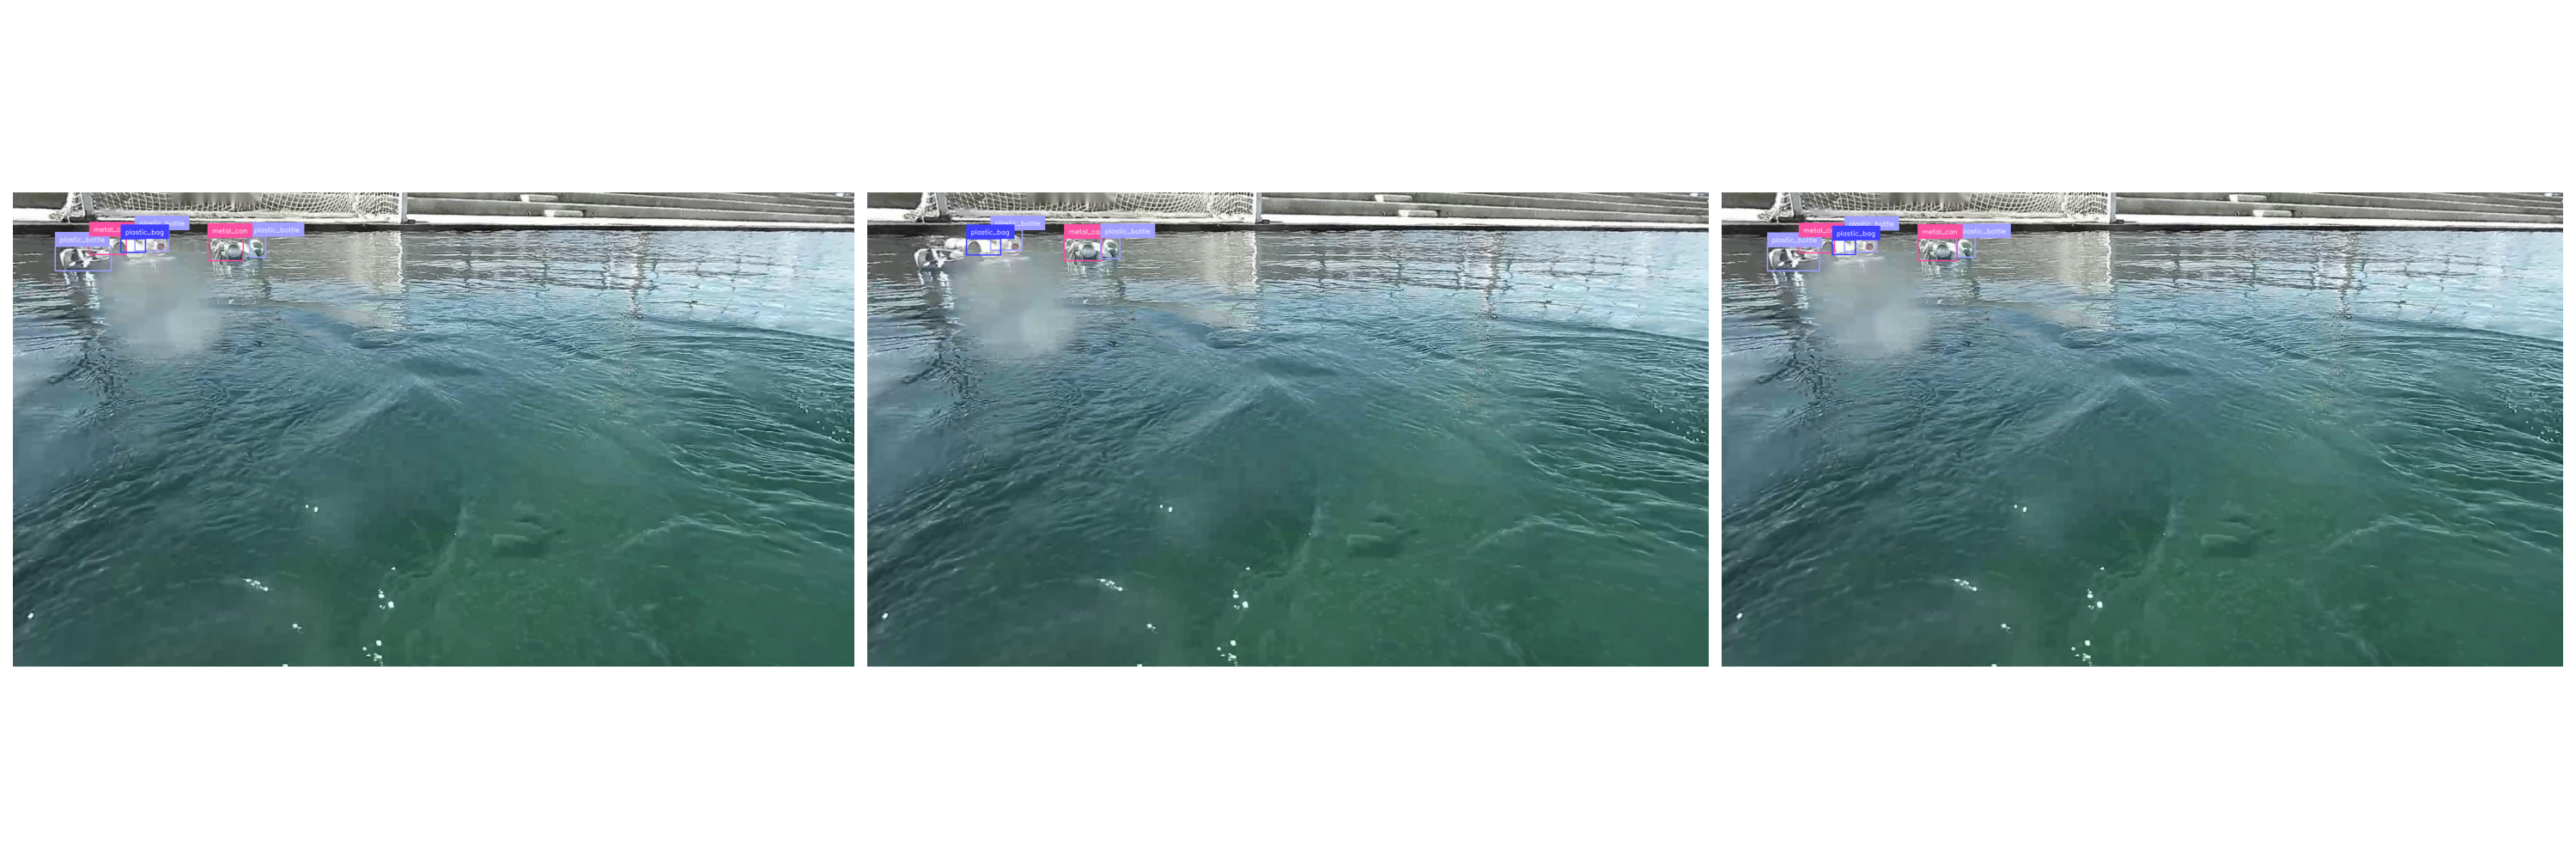
\includegraphics[width=\linewidth]{figures/reflection.png}
		\caption{RF-DETR finds leftmost \textit{bottle} and \textit{can} under glint; YOLO26 misses them.}
		\label{fig:slides-glint}
	\end{figure}
\end{frame}

\begin{frame}{Submergence Test}
	\begin{figure}
		\centering
		{\scriptsize \textbf{Ground Truth} \hspace{3cm} \textbf{YOLO26} \hspace{3cm} \textbf{RF-DETR}} \\
		\vspace{2pt}
		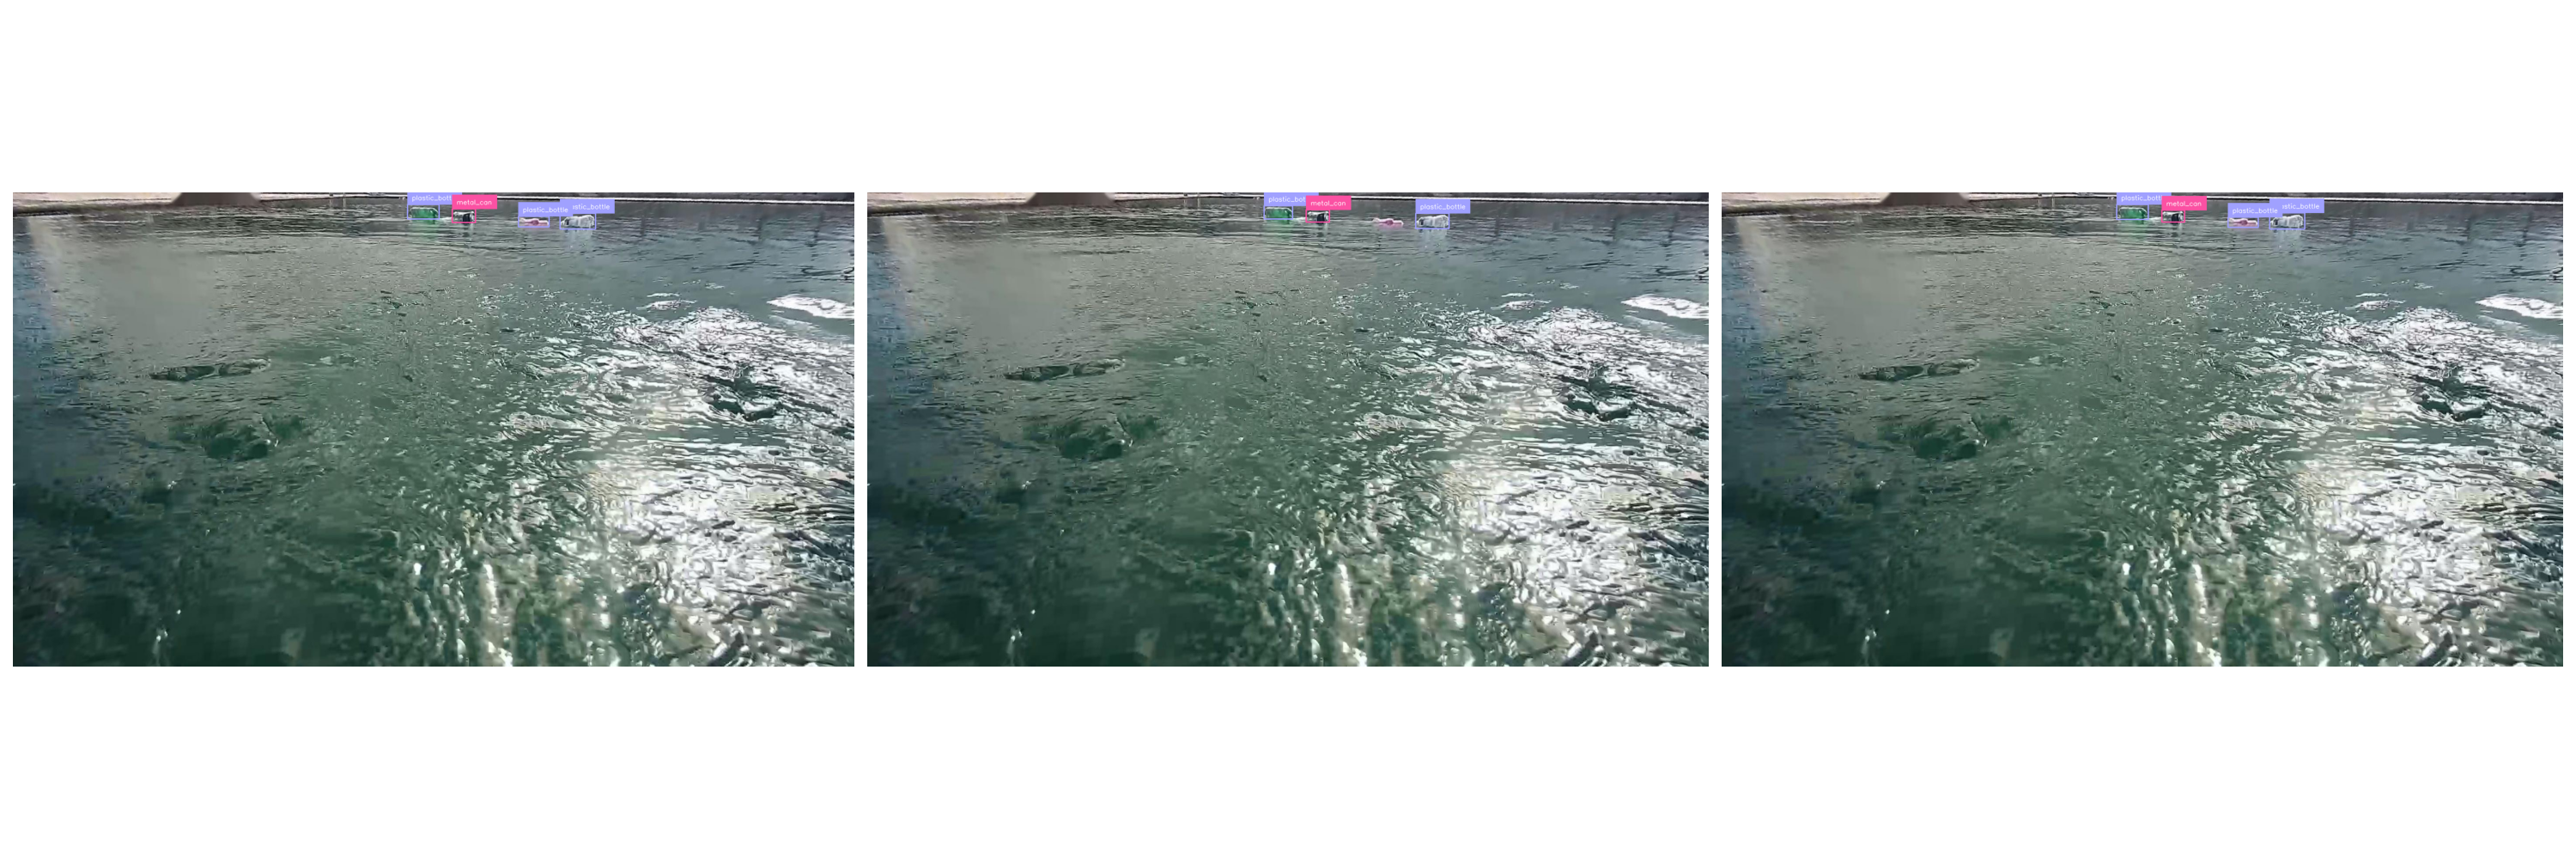
\includegraphics[width=\linewidth]{figures/submerged.png}
		\caption{Partially submerged pink bottle: YOLO26 misses, RF-DETR can identify.}
		\label{fig:slides-submerged}
	\end{figure}
\end{frame}
